\subsection{粒子の回転が系に及ぼす影響}
粒子が系に存在することで生じる応力は,式\eqref{eq:system_stresslet}のように,
それぞれの粒子が存在することによる応力の総和を系の体積で割ることで求めることができる\cite{dilute_squirmer}.
    \begin{equation}
        \boldsymbol{\Sigma}^\mathrm{(p)} = \frac{1}{V} \sum \boldsymbol{S}
        \label{eq:system_stresslet}
    \end{equation}
系に存在する粒子が,squirmer単体である場合には,その存在による応力は,式\eqref{eq:solitary_squirmer_stresslet}のように表される\cite{dilute_squirmer}.
    \begin{equation}
        \boldsymbol{S}_\mathrm{sol} = \frac{4}{3} \pi a^2 (3 \boldsymbol{\hat{e} \cdot \hat{e}} - \boldsymbol{I}) B_2
        \label{eq:solitary_squirmer_stresslet}
    \end{equation}
式\eqref{eq:solitary_squirmer_stresslet}に
式\eqref{eq:orientaion_vector2}を用いて,方向ベクトルを成分表示すると,
    \begin{align}
        \boldsymbol{S}_\mathrm{sol}
        &= \frac{4}{3} \pi a^2
        \left\{
        3
        \left(
            \begin{array}{ccc}
                \sin{\theta} \sin{\theta} & \cos{\theta} \sin{\theta} & 0 \\
                \sin{\theta} \cos{\theta} & \cos{\theta} \cos{\theta} & 0 \\
                0                         & 0                         & 0
            \end{array}
        \right)
        - \left(
            \begin{array}{ccc}
                1 & 0 & 0 \\
                0 & 1 & 0 \\
                0 & 0 & 1
            \end{array}
        \right)
        \right\}
        B_2 \notag \\
        &= \frac{4}{3} \pi a^2 B_2
        \left(
            \begin{array}{ccc}
                3 \sin{\theta} \sin{\theta} - 1 & 3 \cos{\theta} \sin{\theta}     &  0 \\
                3 \sin{\theta} \cos{\theta}     & 3 \cos{\theta} \cos{\theta} - 1 &  0 \\
                0                               & 0                               & -1
            \end{array}
        \right)
        \label{eq:solitary_squirmer_stresslet_elements}
    \end{align}
式\eqref{eq:solitary_squirmer_stresslet_elements}を\eqref{eq:system_stresslet}に代入し,
$xy$成分のみに注目すると式\eqref{eq:stresslet_xy}のように表される.
    \begin{equation}
        \Sigma^\mathrm{(p)}_{xy} = \frac{4 \pi a^2 B_2}{V} \sin{\theta} \cos{\theta}
        \label{eq:stresslet_xy}
    \end{equation}
この応力は,$B_2 > 0$の場合,Fig.\ref{fig:stresslet_xy}のように表される.
    \begin{figure}[H]
        \centering
        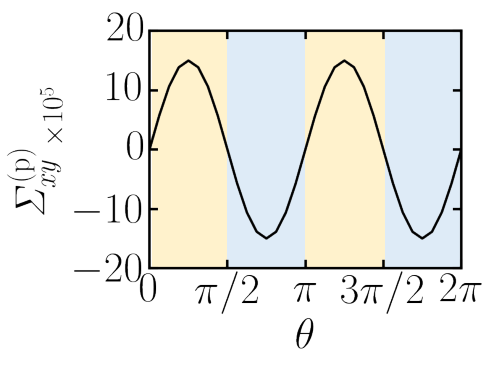
\includegraphics[scale=0.9]{/Users/taiga/Projects/lab/thesis/components/chapter3/figs/bottom_heavy_torque.pdf}
        \caption{単体squirmerの存在による応力の$xy$成分}
        \label{fig:stresslet_xy}
    \end{figure}
\noindent
このグラフより,粒子が定常的に等角速度で回転している場合には,
粒子の存在による応力の時間平均をとると,
プラスとマイナスで打ち消し合い,系に影響は与えないと予想される.
一方,粒子の進行方向がオレンジ色で示した範囲内に固定される場合には,
系の応力を大きくする方向にはたらき,
水色で示した範囲内に固定される場合には,
系の応力を小さくする方向にはたらくことが分かる.
$B_2<0$の場合は逆に,粒子の進行方向がオレンジ色で示した範囲内に固定される場合には,
系の応力を小さくする方向にはたらき,
水色で示した範囲内に固定される場合には,
系の応力を大きくする方向にはたらくことが分かる.
また,粒子が回転する場合でも,
角度によって回転速度が異なる場合には,
応力の時間平均をとってもプラスとマイナスが打ち消さず,
回転速度が小さくなる角度の影響が大きくなることが予想される.
ここで,\ref{sec:purpose}で述べた有効粘度の式を再掲する.
    \begin{equation}
        \eta_\mathrm{eff} = \frac{\sigma}{\dot{\gamma}}
        \tag{\ref{eq:effective_viscosity}}
    \end{equation}
この式から,系にはたらく応力が大きくなると有効粘度は大きくなり,
応力が小さくなると有効粘度は小さくなることがわかる.
したがって,squirmerの存在が系の応力を大きくする方向にはたらく場合は有効粘度も大きくなり,
応力を小さくする方向にはたらく場合には有効粘度も小さくなることが予想される.
\ref{sec:rotation}で述べたように,系のせん断速度がある値よりも小さい場合には,
粒子は回転せずに$0 \leq \theta \leq \pi / 2$の範囲に進行方向が固定されることが予想される.
その場合,$B_2 > 0$のときは,系の応力を大きくする方向にはたらき,
さらに有効粘度も大きくする方向にはたらくと予想される.
逆に,$B_2 < 0$のときは,系の応力および有効粘度を小さくする方向にはたらくと予想される.
また,系のせん断速度がある値よりも大きいとき,
粒子が定常的に回転することが予想されるが,
粒子の等角速度回で回転している場合には,
系の応力および有効粘度には影響を与えないと予想される.
